\documentclass[11pt]{article}

% ---------- Typography & layout ----------
\usepackage[letterpaper,margin=1in]{geometry}
\usepackage[T1]{fontenc}
\usepackage[utf8]{inputenc}
\usepackage{lmodern}
\usepackage{microtype}
\usepackage{setspace}
\usepackage{parskip}

% ---------- Math ----------
\usepackage{amsmath,amssymb,amsthm}
\usepackage{mathtools}

% ---------- Graphics & tables ----------
\usepackage{graphicx}
\usepackage{booktabs}
\usepackage{array}
\usepackage{multirow}
\usepackage{siunitx}
\sisetup{detect-weight=true, detect-family=true, round-mode=places, round-precision=2}

% ---------- Color & links ----------
\usepackage[dvipsnames]{xcolor}
\usepackage[colorlinks=true, linkcolor=blue!50!black, citecolor=blue!50!black, urlcolor=blue!50!black]{hyperref}
\usepackage{cleveref}

% ---------- Bibliography ----------
\usepackage[backend=biber,style=numeric-comp,sorting=none]{biblatex}
\addbibresource{references.bib}

% ---------- Custom notation ----------
\newcommand{\Rips}{\mathrm{VR}}
\newcommand{\Hone}{H_1}
\newcommand{\maxHone}{\ensuremath{\max\text{-}H_1}}

\newcommand{\TODO}[1]{\textcolor{red}{\textbf{[TODO: #1]}}}

\title{\textbf{Does PCA Reveal or Fabricate Topological Structure in Omics Data?}\\
\large A Pre-Registered, Cross-Domain Replication with Matched Null Models}

\author{Santiago Maniches \\ \small TOPOLOGICA LLC \\ \small \href{https://orcid.org/0009-0005-6480-1987}{ORCID: 0009-0005-6480-1987}}

\date{\today}

\begin{document}
\maketitle

\begin{abstract}
Persistent homology applied to PCA-reduced omics data is increasingly invoked as evidence that gene-expression, methylation, or proteomic landscapes contain nontrivial topological structure --- loops, voids, higher-order features --- beyond what a simple cluster or trajectory model would capture. This inference is rarely checked against a null model matched to the same preprocessing pipeline: without one, an apparent $H_1$ (first-homology) signal in PCA space can be a generic artifact of dimensionality reduction on \emph{any} high-dimensional point cloud, real or not. We pre-registered two competing hypotheses --- $H_0^{\text{stat}}$: real-data $\maxHone$ significantly exceeds matched Gaussian and pipeline-symmetric-permutation nulls in both raw and PCA-reduced space; $H_1^{\text{stat}}$: the specific \emph{inflation of persistence induced by PCA} in real data is itself no larger than the inflation the same nulls exhibit --- and tested both across four independent cohorts (five cohort/layer analyses in total, since TCGA-LUAD contributes two omics layers) spanning four tissue types and three omics modalities (bulk RNA-seq, DNA methylation, and mass-spectrometry proteomics): a pilot NSCLC cohort (GSE81089) and three pre-registered confirmatory replications (GSE146889, colorectal/endometrial/ovarian; CPTAC-CCRCC renal proteomics; TCGA-LUAD lung adenocarcinoma RNA-seq and methylation). Across 16 confirmatory BH-FDR-corrected tests, $H_0^{\text{stat}}$ was supported in 14/16 (87.5\%); the two failures occur in a single feature space (TCGA-LUAD methylation after PCA) where the real signal itself collapses to zero. $H_1^{\text{stat}}$ held in its literal, pre-registered form in every cohort tested, and in a stronger directional form (real PCA-delta actually \emph{negative}) in TCGA-LUAD. An 18-configuration ablation sweep on the pilot cohort shows this result is not a fixed-hyperparameter artifact but is bounded: it holds at the pre-registered operating point (2000 highly-variable genes, 50 principal components) and across most of the sampled hyperparameter grid, but breaks down at very low PC counts ($\mathrm{PC}=10$) and, more subtly, at high gene-count/high-PC-count settings (HVG$=4000$, PC$=100$), where the real PCA-driven inflation is comparable to the Gaussian null but no longer to the pipeline-symmetric null.

A further, and separate, question is whether an $H_1$ topological signal --- where one is found to survive both nulls --- reflects a genuine geometric feature of the omics manifold, or is instead a re-description of the tumor/normal class-mean separation already visible to a linear classifier. We built a confound-attribution audit to distinguish the two (within-class decomposition, within-stratum quartile control, residualization against the classifier's own discriminant direction, and block-bootstrap confidence intervals on the residual signal) and applied it to all four cohorts. The result is itself a genuine, dataset-dependent finding rather than a uniform answer: in two cohorts (GSE81089, CPTAC-CCRCC), the $H_1$ signal is not attributable to the tumor/normal class-mean shift by every control tested, including the two most decisive (exact within-class magnitude match; bootstrap CI exclusion of zero), and CPTAC-CCRCC's well-powered normal-tissue arm extends this beyond what the pilot alone could establish. In the other two cohorts (GSE146889, TCGA-LUAD), the picture is materially weaker: GSE146889 passes the within-stratum and aggregate-residualization controls but fails the two most decisive ones, and its dominant topological loop's identity changes after the confound is removed; TCGA-LUAD's signal collapses to null-indistinguishable specifically in the pre-registered PCA(50) space once the confound is removed, the clearest counter-example to a general confound-independence claim in this program. We report this heterogeneity plainly: whether a PCA-space topological signal survives confound control is not a fixed property of the pipeline, but depends on the dataset, and must be tested per dataset rather than assumed from a single successful audit.

\end{abstract}

\section{Introduction}
\label{sec:intro}

Persistent homology (PH) is now a standard tool for characterizing the shape of high-dimensional point clouds, and it has been applied to bulk and single-cell omics data to argue for the presence of loops, branchings, and other topological features that a purely linear or clustering-based analysis would miss~\cite{placeholder-ph-omics}. In a typical workflow, samples are embedded in gene or feature space, reduced via principal component analysis (PCA) to a tractable number of dimensions, and a Vietoris--Rips filtration is built on the resulting point cloud; persistent first-homology ($H_1$) features --- one-dimensional ``loops'' --- are then reported as evidence of nontrivial biological structure: cyclic trajectories, multi-way transitions between cell states, or recurrent sub-populations that PCA has ``revealed.''

This inference has a well-known blind spot. PCA is not merely a projection; on any point cloud, in any number of dimensions, projecting to a lower-dimensional subspace changes the pairwise distance structure and can inflate or deflate persistence values in ways that have nothing to do with the data's substantive structure. When PCA-space $H_1$ persistence is reported as evidence of biological topology, the comparison is almost never made against a null model constructed from the \emph{same} preprocessing pipeline applied to unstructured data. Without that comparison, a claim of the form ``PCA reveals structure'' is unfalsifiable: an equally large signal could arise from resampled noise pushed through the identical highly-variable-gene selection, PCA, and Vietoris--Rips steps.

This project tests two precise, pre-registered, and mutually distinguishable hypotheses against that gap.

\begin{description}
\item[$H_0^{\text{stat}}$ (signal detection).] The maximum $H_1$ persistence observed in real omics data significantly exceeds that of two matched null models --- an i.i.d.\ Gaussian null matched in ambient dimension and sample count, and a pipeline-symmetric permutation null that shuffles each gene's values independently across samples before re-running the identical highly-variable-gene selection, PCA, and filtration steps --- in \emph{both} raw feature space and PCA-reduced space, with effect size $z>3.0$ against both nulls in each space.
\item[$H_1^{\text{stat}}$ (PCA-attribution).] The literal claim tested is narrower and more adversarial to the naive interpretation: does PCA inflate $\maxHone$ in real data by an amount that itself exceeds the inflation the same PCA step induces on null data? If PCA-driven inflation in noise is comparable to or larger than PCA-driven inflation in real signal, then citing a PCA-space $H_1$ feature as evidence of biological topology is not supported by the data --- the inflation itself carries no information.
\end{description}

These two hypotheses are logically independent: a dataset can pass $H_0^{\text{stat}}$ (real data's absolute $\maxHone$ exceeds null) while still failing to license a naive ``PCA reveals structure'' reading if $H_1^{\text{stat}}$'s attribution test shows the PCA step itself is not doing discriminative work. Distinguishing them is the central methodological contribution of this program.

The results reported here rest on three pieces of work, each pre-registered or protocol-locked before analysis: (1) a pilot study (GSE81089, NSCLC bulk RNA-seq) followed by three independent, pre-registered confirmatory replications spanning four tissue types and two additional omics modalities (DNA methylation, mass-spectrometry proteomics); (2) an 18-configuration ablation sweep over the pilot cohort's hyperparameters (highly-variable-gene count, PCA component count, permutation count, missing-value imputation rule) to establish the boundary of the pre-registered operating point's validity; and (3) a confound-attribution audit designed to test whether an $H_1$ signal that does survive both nulls is a genuine feature of the omics manifold or merely a re-encoding of the tumor/normal class-mean separation that a linear classifier can already recover at near-ceiling accuracy in every cohort tested.

We treat the third question --- confound attribution --- as open rather than resolved. The audit protocol has so far been executed to completion only on the pilot cohort, where it finds the topological signal is not attributable to the class-mean shift; whether this holds in the three replication cohorts is a live, unanswered question that this paper tests but does not yet close, and one of the confirmatory cohorts (GSE146889) already shows a structural reason for caution: its dominant $H_1$ loop is significantly enriched for tumor-status samples, unlike the pilot's loop, meaning confound-independence found in one cohort should not be assumed to transfer to another without direct testing. \TODO{final synthesis of confound-audit generalization across all four cohorts to be inserted once the remaining three audits complete}

The remainder of the paper proceeds as follows. \Cref{sec:methods} describes the persistent-homology and null-model pipeline, the five cohorts and their two additional omics modalities, the ablation sweep design, and the confound-attribution audit protocol. \Cref{sec:results} reports the cross-dataset $H_0^{\text{stat}}$/$H_1^{\text{stat}}$ replication results, the ablation sweep's hyperparameter-sensitivity boundary, and the pilot-cohort confound-audit finding. \Cref{sec:discussion} synthesizes these results into a scope statement for what this program does and does not establish. \TODO{Discussion section to be finalized once confound-audit generalization results are available}

\section{Methods}
\label{sec:methods}

\subsection{Pre-registration discipline}

All primary hyperparameters, normalization rules, effect-size thresholds, and the confirmatory dataset family were locked in a pre-registration document (\texttt{PREREGISTRATION.md}) prior to any confirmatory analysis, timestamped and accompanied by a SHA-256 hash recorded at lock time as an internal provenance marker (the hash was computed over the document's content immediately before the hash line itself was appended, so it is not independently recomputable from the committed file as currently stored; it is retained here as a record of the locking procedure followed, not as a reader-verifiable checksum). The pilot cohort (GSE81089) was used to develop the pipeline and is reported separately from the confirmatory family; only the three subsequently-analyzed cohorts (GSE146889, CPTAC-CCRCC, TCGA-LUAD) contribute to the pre-registered, multiple-testing-corrected confirmatory statistics reported in \Cref{sec:results}. The decision rule fixed in advance was that each dataset's result stands on its own merits --- a dataset that fails a gate (e.g., the intrinsic-dimension check below) is reported as blocked or deviated, not silently dropped from the family.

\subsection{Persistent homology pipeline}

For each cohort and omics layer, samples are represented as points in a feature space (genes, methylation probes, or proteins). Two feature spaces are analyzed per cohort/layer: (i) \emph{raw} space, restricted to the top highly-variable features (HVG count fixed at 2000 in the pre-registered configuration; varied in the ablation sweep, \Cref{sec:methods-ablation}); and (ii) \emph{PCA-reduced} space, obtained by projecting the raw feature matrix onto its top 50 principal components (varied in the ablation sweep). A Vietoris--Rips filtration $\Rips(X,\varepsilon)$ is built on the resulting point cloud $X$ in each space, and persistent $H_1$ features are computed; the primary test statistic throughout is $\maxHone$, the longest-lived $H_1$ bar (death $-$ birth) in each filtration. This choice --- a single scalar summary rather than a full persistence-diagram distance (e.g.\ bottleneck or Wasserstein) --- was fixed at pre-registration to keep the statistical comparison against null distributions simple and the effect-size definition unambiguous.

\subsection{Null models}

Two null models are computed in parallel, matched to the same feature space and sample count as the real data at each step:

\begin{description}
\item[Gaussian null.] 500 draws of i.i.d.\ Gaussian noise, dimension- and sample-count-matched to the real data, independently subjected to the identical HVG-selection (where applicable), PCA, and Rips-filtration pipeline as the real data.
\item[Pipeline-symmetric permutation null.] 2000 permutations in which each gene/feature's values are independently shuffled across samples (destroying all cross-feature correlation structure while preserving each feature's marginal distribution exactly), then re-run through the identical HVG-selection, PCA, and filtration pipeline.
\end{description}

The permutation null is the more conservative and more relevant comparison for the $H_1^{\text{stat}}$ (PCA-attribution) test, since it inherits the real data's marginal feature distributions exactly and differs from the real data only in cross-feature dependence structure --- any $\maxHone$ inflation it shows under PCA is attributable purely to the projection step acting on realistic per-feature marginals, not to a mismatched noise model. Both nulls are retained throughout because they answer different questions: the Gaussian null asks whether the signal exceeds what unstructured continuous noise would produce; the permutation null asks whether it exceeds what the same marginal distributions, decorrelated, would produce.

Permutation-count convergence was checked in the ablation sweep (\Cref{sec:methods-ablation}): $z$-scores versus the pipeline-symmetric null were computed at $n_{\text{perm}} \in \{100, 250, 500, 1000, 2000\}$ and found to have converged (bootstrapped 95\% CI stabilized) well before the pre-registered $n=2000$.

\subsection{Effect size and significance thresholds}

Effect size against each null is reported as a $z$-score: $(\text{observed} - \text{null mean})/\text{null SD}$. The pre-registered significance threshold is $z>3.0$ in every comparison (both null models, both feature spaces), chosen to clear the pilot's weakest single margin with room to spare while remaining well above conventional large-effect benchmarks. For the confirmatory family (GSE146889, CPTAC-CCRCC, TCGA-LUAD), the resulting $p$-values across up to 20 planned tests are corrected for multiple comparisons via Benjamini--Hochberg FDR control at $\alpha=0.05$~\cite{benjaminihochberg1995}; a test is reported as passing $H_0^{\text{stat}}$ only if it clears both the raw $z>3.0$ threshold and the BH-adjusted significance criterion.

\subsection{Intrinsic dimension and Johnson--Lindenstrauss regime gate}

Before PCA is applied, the intrinsic dimensionality of each feature space is estimated using two independent estimators --- the Levina--Bickel maximum-likelihood estimator~\cite{levinabickel2004} and the TwoNN estimator~\cite{facco2017} --- and compared against the ambient (post-HVG) dimension. When the ratio $d_{\text{int}}/d_{\text{amb}} \geq 0.3$, the data is judged to sit outside the regime in which Euclidean Vietoris--Rips distances behave predictably under linear projection (the Johnson--Lindenstrauss heuristic~\cite{johnsonlindenstrauss1984} is not expected to hold), and a spectral-cascade metric --- in the spirit of recent spectral-distance approaches to persistent homology on high-dimensional, low-intrinsic-dimension data~\cite{damrich2024} --- is substituted for the naive Euclidean distance in that space's filtration. This gate was triggered for TCGA-LUAD's methylation PCA space ($d_{\text{int}}/d_{\text{amb}} = 0.320$; \Cref{sec:results}), where it is flagged as a pre-registered deviation rather than an ad hoc fix.

\subsection{Datasets}

Five cohorts, spanning four tissue/tumor types and three omics modalities, were analyzed:

\begin{itemize}
\item \textbf{GSE81089} (pilot, not part of the confirmatory family): NSCLC bulk RNA-seq, $n=218$ (199 tumor / 19 normal).
\item \textbf{GSE146889}: colorectal/endometrial/ovarian MMR-deficiency cohort, bulk RNA-seq, $n=176$ (91 tumor / 85 paired-normal).
\item \textbf{CPTAC-CCRCC} (PDC000127): renal clear-cell carcinoma, mass-spectrometry proteomics, $n=194$ (110 tumor / 84 normal), no substitution required.
\item \textbf{TCGA-LUAD}: lung adenocarcinoma, two omics layers --- RNA-seq ($n=116$) and DNA methylation ($n=36$ paired samples, 58 cases with both layers available).
\end{itemize}

Normalization follows modality-specific pre-registered rules: bulk RNA-seq is $\log_1p$-transformed (FPKM or TPM as available per cohort); DNA methylation is logit-transformed on the $\beta$-value scale (clipped to $[10^{-6}, 1-10^{-6}]$ to avoid boundary singularities); CPTAC proteomics is median-normalized then $\log_2$-transformed. Missing values are zero-filled in the pre-registered primary analysis; three alternative imputation rules (mean, median, drop) are compared in the ablation sweep (\Cref{sec:methods-ablation}).

TCGA-LUAD required four declared deviations from the pre-registered protocol, each pre-specified as a contingency rather than an ad hoc decision after seeing results: (D1) the ``bottom-variance'' negative-control gene set is selected among genes with nonzero variance only (5{,}556 of 60{,}660 genes have exactly zero variance and would trivially fail any test); (D2) methylation $\beta$-values are clipped before the logit transform; (D3) methylation PCA is capped at 35 components rather than the pre-registered 50, since only 35 are available given the sample count, and is treated as a rotation-only isometry check rather than an independent significance test; (D4) the spectral-cascade metric is applied to the methylation PCA space per the intrinsic-dimension gate above.

\subsection{Ablation / hyperparameter-sensitivity sweep}
\label{sec:methods-ablation}

To establish the boundary of validity around the pre-registered operating point (HVG$=2000$, PC$=50$), an 18-configuration sweep was run on the pilot cohort (GSE81089), varying: HVG gene count ($\{500, 1000, 2000, 4000\}$, PC count fixed at 50); PCA component count ($\{10, 25, 50, 100\}$, HVG fixed at 2000); missing-value imputation rule (zero, mean, median, drop); and a $2\times2$ gene-count $\times$ PC-count interaction check at the corners of the grid (HVG$\in\{500,4000\}$ $\times$ PC$\in\{10,100\}$) to test whether the two hyperparameters' effects are additive or interact superadditively. Permutation count was reduced to $n=500$ in the sweep (from the pre-registered $n=2000$) to keep the 18-configuration sweep computationally tractable; convergence at this reduced count was separately verified (above).

\subsection{Confound-attribution audit protocol}
\label{sec:methods-confound}

Where an $H_1^{\text{stat}}$ signal is found to survive both null models, a separate question is whether that signal reflects genuine topological structure in the omics manifold, or is instead a re-description of the tumor/normal class-mean separation --- a shift that a simple linear classifier can already recover, in every cohort tested here, at or near ceiling cross-validated AUC. The audit protocol, applied here to all four cohorts (\Cref{sec:results-confound}, \Cref{sec:results-confound-generalization}), consists of four complementary checks:

\begin{enumerate}
\item \textbf{Within-class decomposition.} The $\maxHone$ statistic is recomputed on the tumor-only subpopulation alone (excluding normal samples entirely), and separately on the normal-only subpopulation. If the mixed-population signal is driven purely by the tumor/normal class-mean gap, it should collapse when either subpopulation is analyzed in isolation.
\item \textbf{Within-stratum control.} The tumor-only subpopulation is further stratified into quartiles along the direction of maximal tumor/normal class-mean separation (the top discriminant axis, e.g.\ PC1 where correlated with class), and the $H_1^{\text{stat}}$ test is repeated within each quartile. A signal that survives uniformly across quartiles cannot be attributed to residual variation along that specific confound direction.
\item \textbf{Residualization control.} The tumor/normal class-mean-shift direction is estimated and projected out of the feature matrix (residualization), and the $H_1^{\text{stat}}$ test is repeated on the residualized data. A 5-fold cross-validated logistic regression classifier trained to recover tumor/normal status from the residualized data is also evaluated; its cross-validated AUC collapsing toward chance is evidence the confound direction has been successfully removed without also removing the topological signal. We note that linear confound-regression procedures of this kind have themselves been shown, in other machine-learning contexts, to introduce leakage or distort downstream nonlinear statistics rather than cleanly removing the confound~\cite{hamdan2023}; we do not use a nonlinear downstream model here (only the linear residual's own topology and a linear classifier check), which limits but does not eliminate this concern (\Cref{sec:discussion}).
\item \textbf{Block-bootstrap confidence interval.} A block-bootstrap procedure (resampling at the sample level, preserving each feature's within-sample structure) is used to construct a 95\% confidence interval on the residual signal-beyond-null quantity after residualization; an interval excluding zero is evidence the residual signal is not a bootstrap artifact of the small effective sample size in some strata.
\end{enumerate}

This protocol was applied identically across all four cohorts (\Cref{sec:results-confound}, \Cref{sec:results-confound-generalization}). GSE146889's own replication report had already surfaced a specific structural reason its result might diverge from the pilot's: its dominant $H_1$ loop is significantly enriched for tumor-status samples (Fisher's exact $p=2.9\times10^{-9}$), unlike the pilot's small, non-enriched loop; the audit confirms this concern is real, though only partially, rather than resolving it in either direction.

\section{Results}
\label{sec:results}

\subsection{Pilot cohort: motivating result}

In the pilot cohort (GSE81089, NSCLC bulk RNA-seq, $n=218$), real data's $\maxHone$ significantly exceeds both null models in raw feature space ($z=26.1$ vs.\ Gaussian, $z=14.9$ vs.\ pipeline-symmetric permutation) and in PCA(50)-reduced space ($z=5.19$ vs.\ Gaussian, $z=5.23$ vs.\ permutation), supporting $H_0^{\text{stat}}$ in this cohort. However, the PCA-driven increase in $\maxHone$ observed in the real data ($\Delta = 0.78$) is \emph{smaller} than the PCA-driven increase observed in either null model applied to the same pipeline (Gaussian null $\Delta = 2.00 \pm 0.34$; pipeline-symmetric null $\Delta = 1.50 \pm 0.39$), i.e.\ PCA inflates persistence in unstructured noise \emph{more} than it does in the real NSCLC data. This is the pilot's motivating finding for $H_1^{\text{stat}}$ and is shown in \Cref{fig:fig1}: naive reporting of the PCA-space $H_1$ feature alone, without this comparison, would have overstated the topological claim.

\begin{figure}[htbp]
\centering
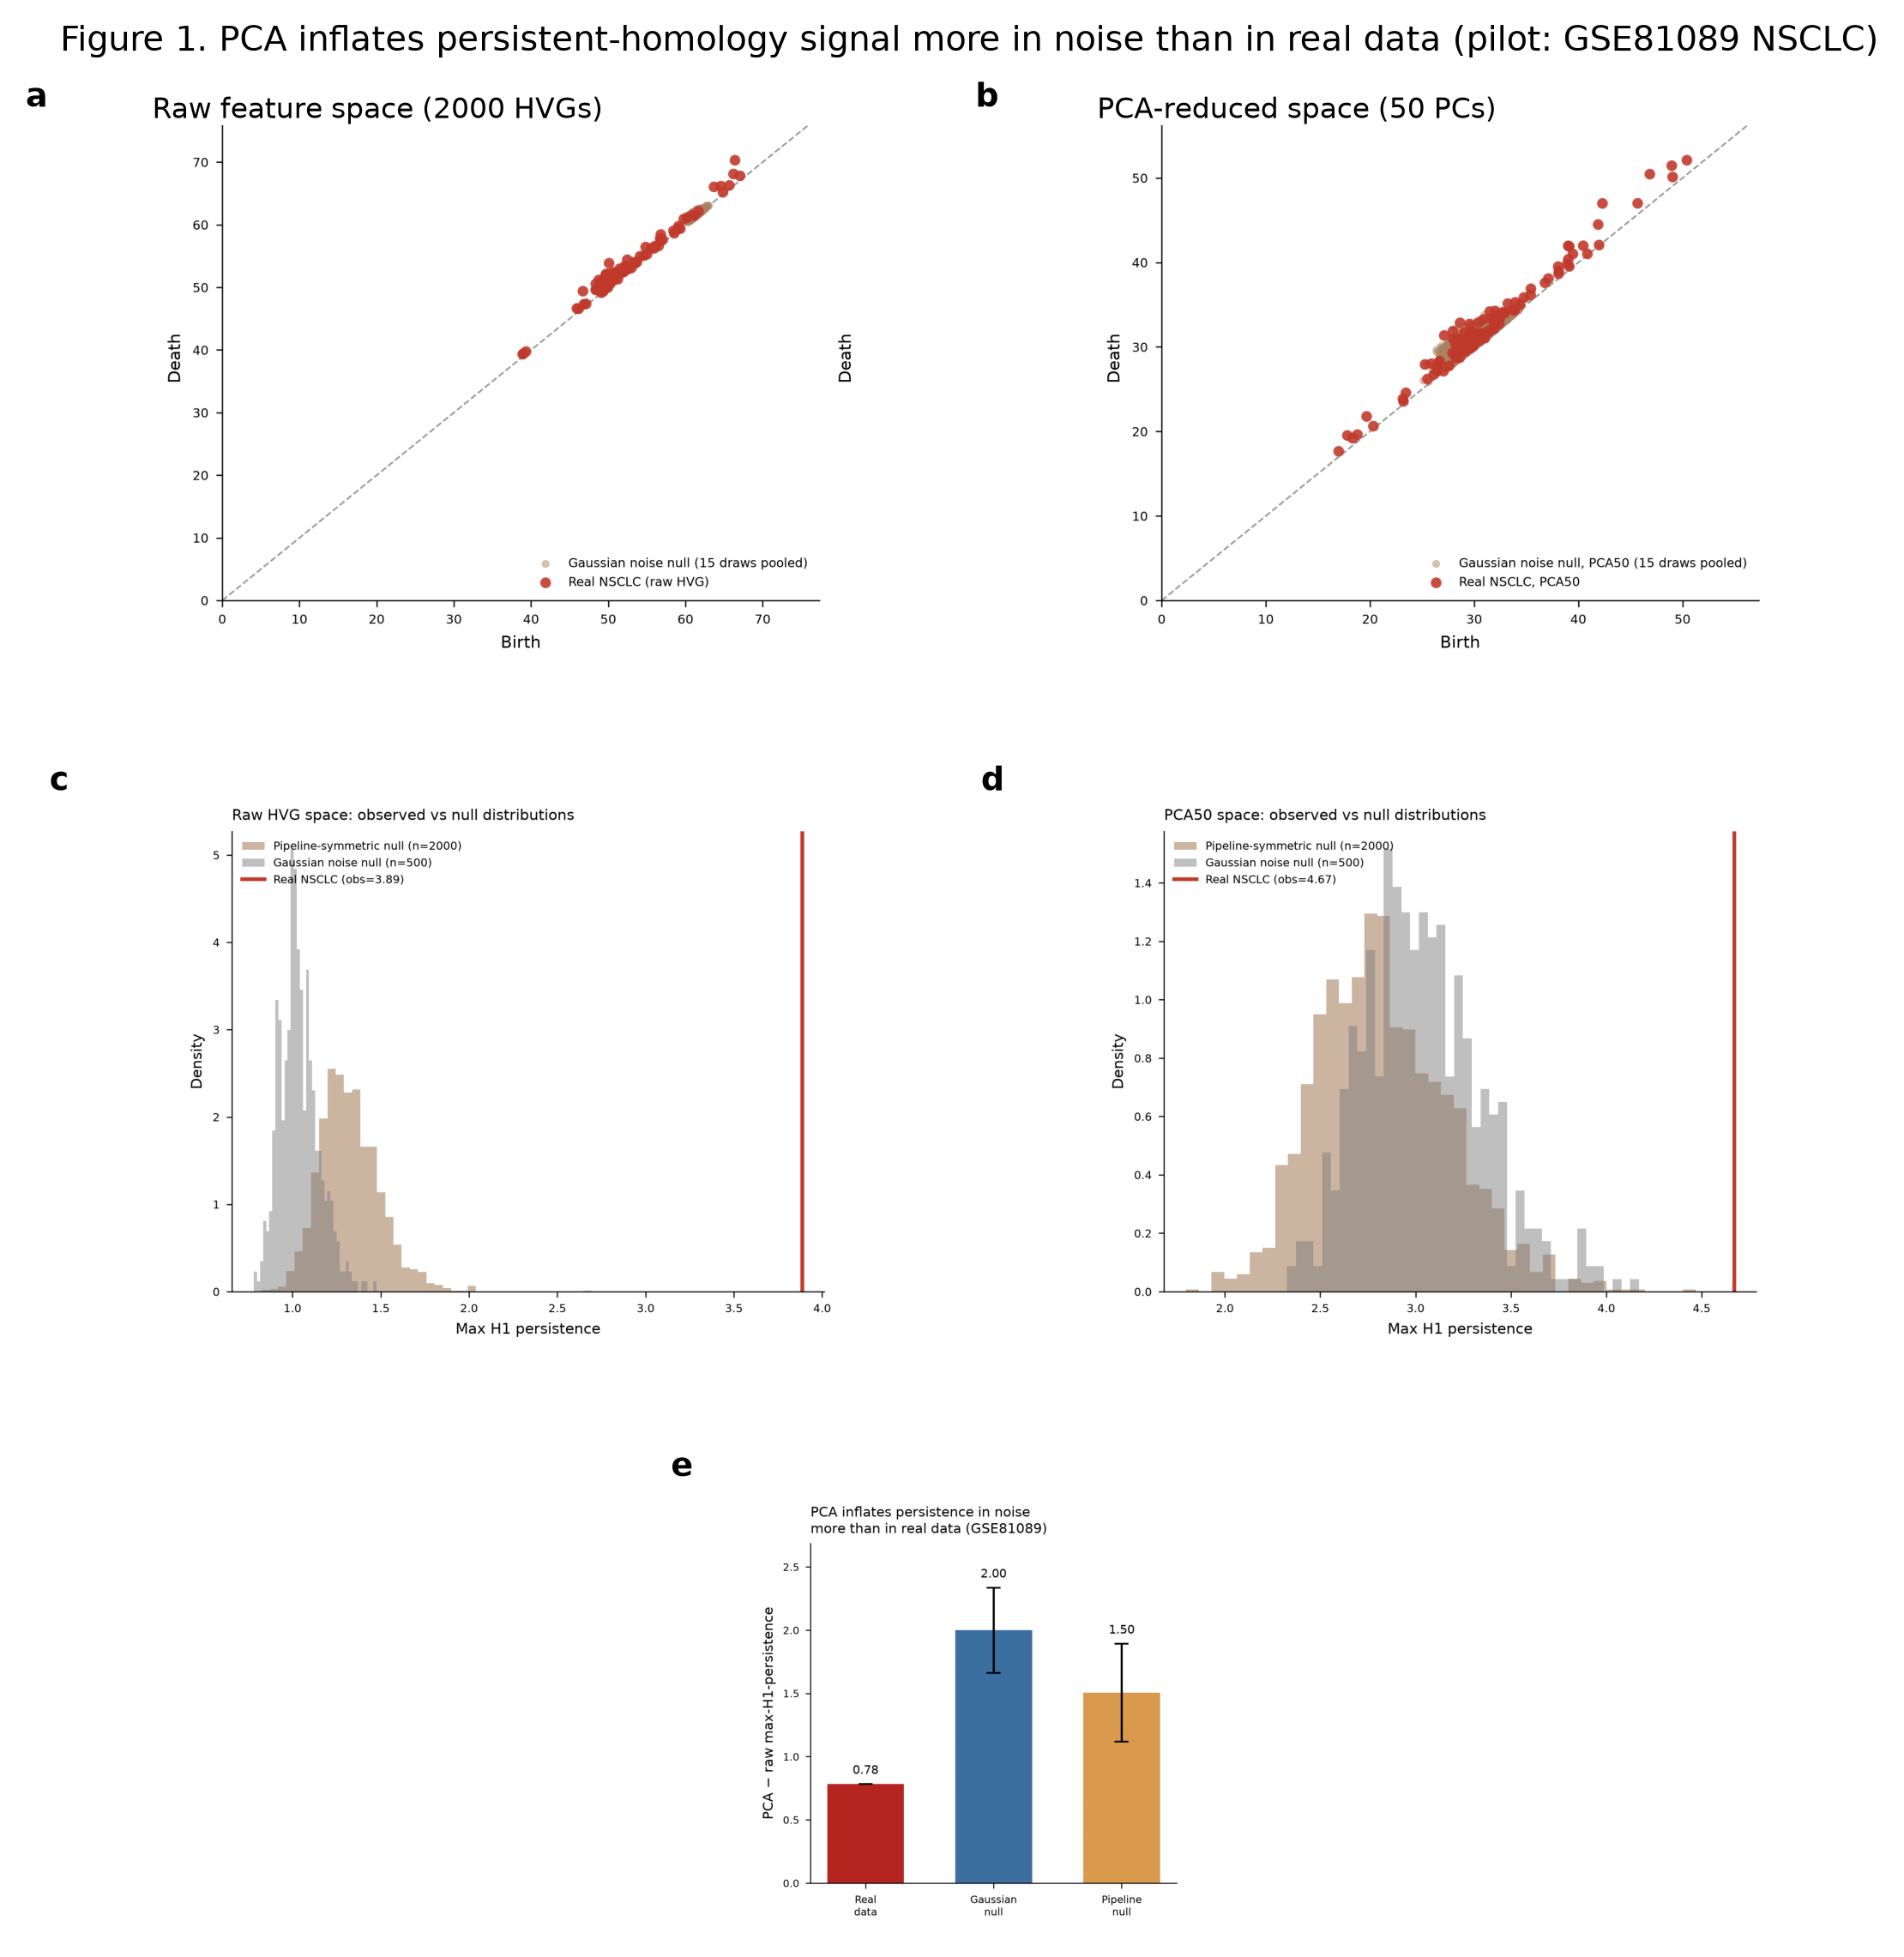
\includegraphics[width=0.95\textwidth]{figures/fig1_pilot_motivation.png}
\caption{\textbf{PCA amplifies persistent-homology signal in noise as much as in real data (pilot cohort, GSE81089 NSCLC).} (a--b) $H_1$ persistence diagrams, real data (red) vs.\ pooled Gaussian-noise null (tan), in raw feature space (a) and PCA(50)-reduced space (b); real points shift further above the diagonal in PCA space, but so does the null. (c--d) Observed $\maxHone$ (vertical red line) against the pipeline-symmetric permutation null (tan) and Gaussian null (grey) distributions, in raw (c) and PCA (d) space; real data exceeds both nulls by a wide margin in both spaces ($H_0^{\text{stat}}$ supported). (e) The PCA-driven $\Delta$ in $\maxHone$ is smaller in real data (0.78) than in either null model (Gaussian: 2.00; pipeline-symmetric: 1.50), showing PCA's persistence-inflating effect on this cohort's noise floor is larger than its effect on the real signal.}
\label{fig:fig1}
\end{figure}

\subsection{Cross-dataset replication}

The three confirmatory cohorts (GSE146889, CPTAC-CCRCC, TCGA-LUAD) contribute 16 pre-registered, BH-FDR-corrected tests of $H_0^{\text{stat}}$ (\Cref{tab:h0-crossdataset}). 14 of 16 (87.5\%) pass at BH-adjusted $\alpha=0.05$ and the pre-registered $z>3.0$ threshold. The two failures are both in the same feature space: TCGA-LUAD's methylation data, after PCA(35, spectral metric), shows real $\maxHone$ collapsing to zero, so neither the Gaussian ($z=-0.20$) nor permutation ($z=-0.79$) comparison can register a signal --- this is a failure of the real signal to survive PCA in that specific modality, not a failure of the null models.

\begin{table}[htbp]
\centering
\small
\caption{$H_0^{\text{stat}}$ cross-dataset replication: $z$-scores vs.\ matched nulls, raw and PCA-reduced space. All effect sizes clear $z>3.0$ except TCGA-LUAD methylation PCA (both nulls).}
\label{tab:h0-crossdataset}
\begin{tabular}{@{}llrrl@{}}
\toprule
Dataset & Layer / space & $z$ (Gaussian) & $z$ (permutation) & BH-corrected pass \\
\midrule
GSE81089 (pilot)\footnotemark[1] & RNA-seq, raw & 26.06 & 14.92 & --- \\
GSE81089 (pilot)\footnotemark[1] & RNA-seq, PCA50 & 5.19 & 5.23 & --- \\
GSE146889 & RNA-seq, raw & 44.87 & 39.59 & Yes \\
GSE146889 & RNA-seq, PCA50 & 12.02 & 11.37 & Yes \\
CPTAC-CCRCC & Proteomics, raw & 23.18 & 21.39 & Yes \\
CPTAC-CCRCC & Proteomics, PCA50 & 4.40 & 4.64 & Yes \\
TCGA-LUAD & RNA-seq, raw & 58.67 & 47.53 & Yes \\
TCGA-LUAD & RNA-seq, PCA50 & 9.19 & 8.34 & Yes \\
TCGA-LUAD & Methylation, raw & 19.34 & 26.69 & Yes \\
TCGA-LUAD & Methylation, PCA35 (spectral) & $-0.20$ & $-0.79$ & \textbf{No} \\
\bottomrule
\end{tabular}
\vspace{2pt}
\footnotesize{\footnotemark[1]Pilot cohort shown for reference; not part of the pre-registered confirmatory BH-FDR family.}
\end{table}

Table~\ref{tab:h1-crossdataset} reports the $H_1^{\text{stat}}$ (PCA-attribution) comparison in every cohort and layer: the real PCA-driven $\Delta$ in $\maxHone$ against the range spanned by the two null models' own PCA-driven $\Delta$. In GSE81089, GSE146889, and CPTAC-CCRCC, the real $\Delta$ is positive but smaller than both null $\Delta$s --- the pre-registered, literal form of $H_1^{\text{stat}}$ holds in each. TCGA-LUAD RNA-seq shows a stronger form of the same conclusion: the real $\Delta$ is \emph{negative} ($-0.89$), i.e.\ PCA in this cohort's RNA-seq layer actually \emph{reduces} $\maxHone$ relative to raw space, while both nulls show a positive inflation of $+2.35$ to $+2.51$ --- an even larger gap disfavoring the naive interpretation. TCGA-LUAD's methylation layer is a distinct case: the real $\Delta$ is strongly negative ($-4.09$), driven by the real signal's near-total collapse under PCA(35, spectral) noted above, while the null $\Delta$s are mildly negative ($-0.90$ to $-0.79$); this is consistent with $H_1^{\text{stat}}$ but for a different underlying reason (loss of real signal rather than a comparable but smaller inflation).

\begin{table}[htbp]
\centering
\small
\caption{$H_1^{\text{stat}}$ cross-dataset replication: real PCA-driven $\Delta$(max-$H_1$) vs.\ range spanned by null models' own $\Delta$.}
\label{tab:h1-crossdataset}
\begin{tabular}{@{}lrrl@{}}
\toprule
Dataset / layer & Real $\Delta$ & Null $\Delta$ range & $H_1^{\text{stat}}$ verdict \\
\midrule
GSE81089 (pilot) & $+0.78$ & $[1.50, 2.00]$ & Supported \\
GSE146889 & $+1.36$ & $[2.08, 2.18]$ & Supported \\
CPTAC-CCRCC & $+0.85$ & $[2.01, 2.10]$ & Supported \\
TCGA-LUAD RNA-seq & $-0.89$ & $[2.35, 2.51]$ & Supported (stronger form) \\
TCGA-LUAD Methylation & $-4.09$ & $[-0.90, -0.79]$ & Supported (distinct mechanism) \\
\bottomrule
\end{tabular}
\end{table}

\Cref{fig:fig2} summarizes both tables graphically alongside the confound cross-check (\Cref{sec:results-confound-crossdataset}).

\begin{figure}[htbp]
\centering
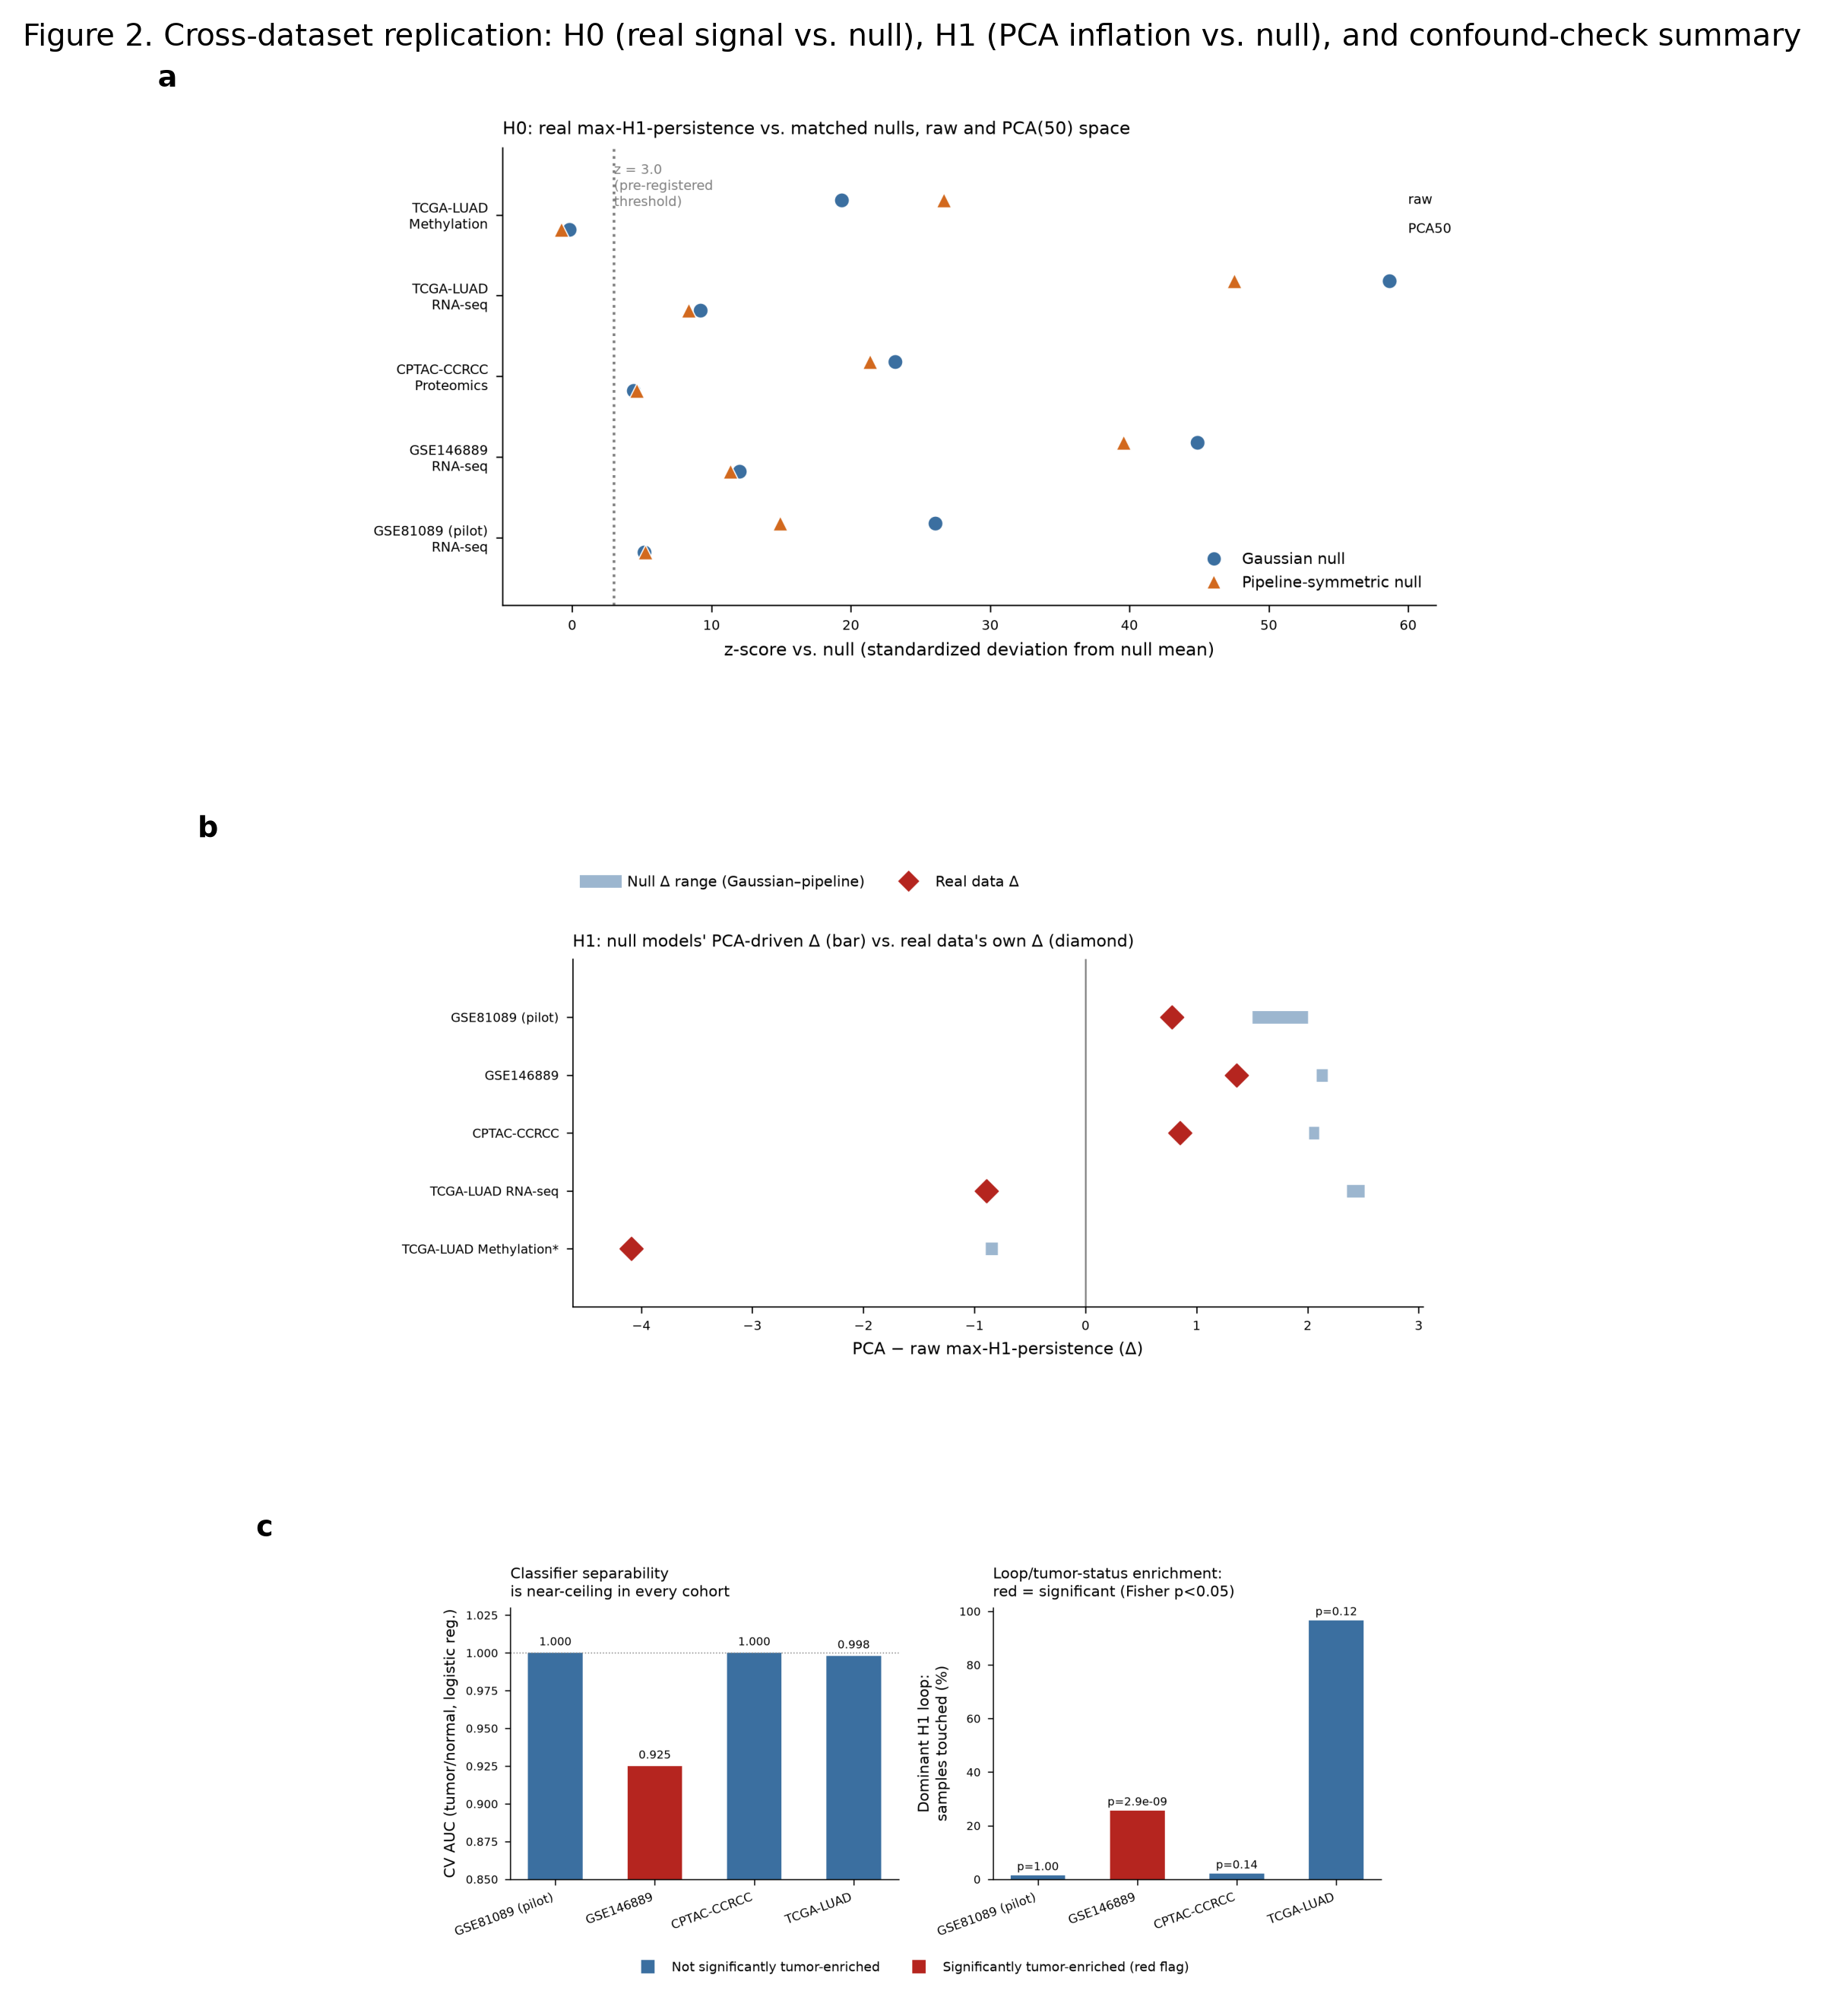
\includegraphics[width=0.92\textwidth]{figures/fig2_cross_dataset_replication.png}
\caption{\textbf{Cross-dataset replication summary.} (a) $H_0^{\text{stat}}$: $z$-scores of real $\maxHone$ vs.\ Gaussian (circle) and pipeline-symmetric (triangle) nulls, raw and PCA(50) space, across all five cohort/layer combinations; dotted line marks the pre-registered $z=3.0$ threshold. All comparisons clear threshold except TCGA-LUAD methylation PCA space. (b) $H_1^{\text{stat}}$: real PCA-driven $\Delta$ in $\maxHone$ (diamond) against the range spanned by the two null models' own PCA-driven $\Delta$ (bar); real $\Delta$ falls at or below the null range in every cohort. (c) Confound cross-check: cross-validated classifier AUC for tumor/normal status (left) and the fraction of samples touched by the dominant $H_1$ loop, colored by whether that loop is significantly enriched for tumor status (Fisher's exact test, right). GSE146889 is flagged red: its loop is significantly tumor-enriched, unlike the other three cohorts.}
\label{fig:fig2}
\end{figure}

\subsection{Confound cross-check across cohorts}
\label{sec:results-confound-crossdataset}

Independent of the full confound-\emph{attribution} audit (\Cref{sec:methods-confound}, applied to date only to the pilot cohort), each replication report includes a lighter cross-check: cross-validated tumor/normal classifier AUC, and whether the dominant $H_1$ loop's participating samples are significantly enriched for one class (Fisher's exact test). Classifier AUC is at or near ceiling in every cohort (GSE81089: 1.000; GSE146889: 0.925; CPTAC-CCRCC: 1.000; TCGA-LUAD: 0.918--0.998 across spaces) --- the tumor/normal distinction is linearly separable everywhere, which is precisely why the confound-attribution question in \Cref{sec:methods-confound} is worth asking at all. The dominant-loop enrichment check, however, differs sharply across cohorts: GSE81089's loop touches only 3/218 samples and is not significantly enriched (Fisher $p=1.0$); CPTAC-CCRCC's loop touches 3--4/194 samples, also not significant ($p>0.13$); TCGA-LUAD's loop touches 112/116 samples (essentially the whole cohort) and is not significantly enriched relative to overall tumor fraction ($p=0.12$). GSE146889 is the exception: its dominant loop touches 45/176 samples and \emph{is} significantly enriched for tumor status (odds ratio 12.5, Fisher $p=2.9\times10^{-9}$) --- a structurally different pattern from the pilot's clean, non-enriched loop, and the specific reason the pilot's confound-audit conclusion (\Cref{sec:results-confound}) cannot be assumed to generalize to GSE146889 without direct testing.

\subsection{Ablation / hyperparameter-sensitivity sweep}

The 18-configuration sweep on the pilot cohort (\Cref{fig:fig3}) shows $H_1^{\text{stat}}$ is directionally robust at the pre-registered operating point (HVG$=2000$, PC$=50$) and across most of the sampled grid (14/18 configurations, 78\%, support $H_1^{\text{stat}}$ against both nulls simultaneously; $H_0^{\text{stat}}$ holds in 16/18, 89\%), but fails in two distinct, identifiable regimes:

\begin{enumerate}
\item \textbf{Low PC count (PC=10), dominant failure mode.} At PC$=10$, across all three HVG settings tested at that PC count (500, 2000, 4000), the real PCA-driven $\Delta$ (1.36--5.65) exceeds \emph{both} null models' $\Delta$ --- the direction of the pre-registered $H_1^{\text{stat}}$ inequality reverses. Aggressive dimensionality reduction to very few components appears to let the real data's structure dominate the projection in a way the null pipeline does not reproduce at the same PC count.
\item \textbf{High gene-count / high PC-count (HVG=4000, PC=100), secondary failure mode.} At this corner, the real $\Delta$ (2.45) exceeds the pipeline-symmetric null's $\Delta$ (2.36) --- $H_1^{\text{stat}}$ fails specifically against the more conservative permutation null, despite highly significant $z$-scores against the null distributions overall (raw-space $z=20.4$ vs.\ pipeline, $z=28.2$ vs.\ Gaussian) --- while still passing against the Gaussian null ($\Delta=2.75$).
\end{enumerate}

Permutation count converged well before the pre-registered $n=2000$ (bootstrapped 95\% CI on the $z$-score stabilizes by $n\approx250$--$500$ for both raw- and PCA-space comparisons). Missing-value imputation rule is essentially inconsequential to the HVG selection at the pre-registered operating point: pairwise Jaccard overlap of the selected highly-variable gene sets across all four rules (zero, mean, median, drop) is $\geq0.97$, and all four rules agree on which samples participate in the dominant $H_1$ loop (Jaccard $=1.000$). The gene-count $\times$ PC-count interaction check (\Cref{fig:fig3}b) finds the observed joint effect exceeds the additive (leave-one-out-summed) prediction from each hyperparameter's marginal effect at all four grid corners, indicating a genuine superadditive interaction rather than two independent, additive nuisance effects.

\begin{figure}[htbp]
\centering
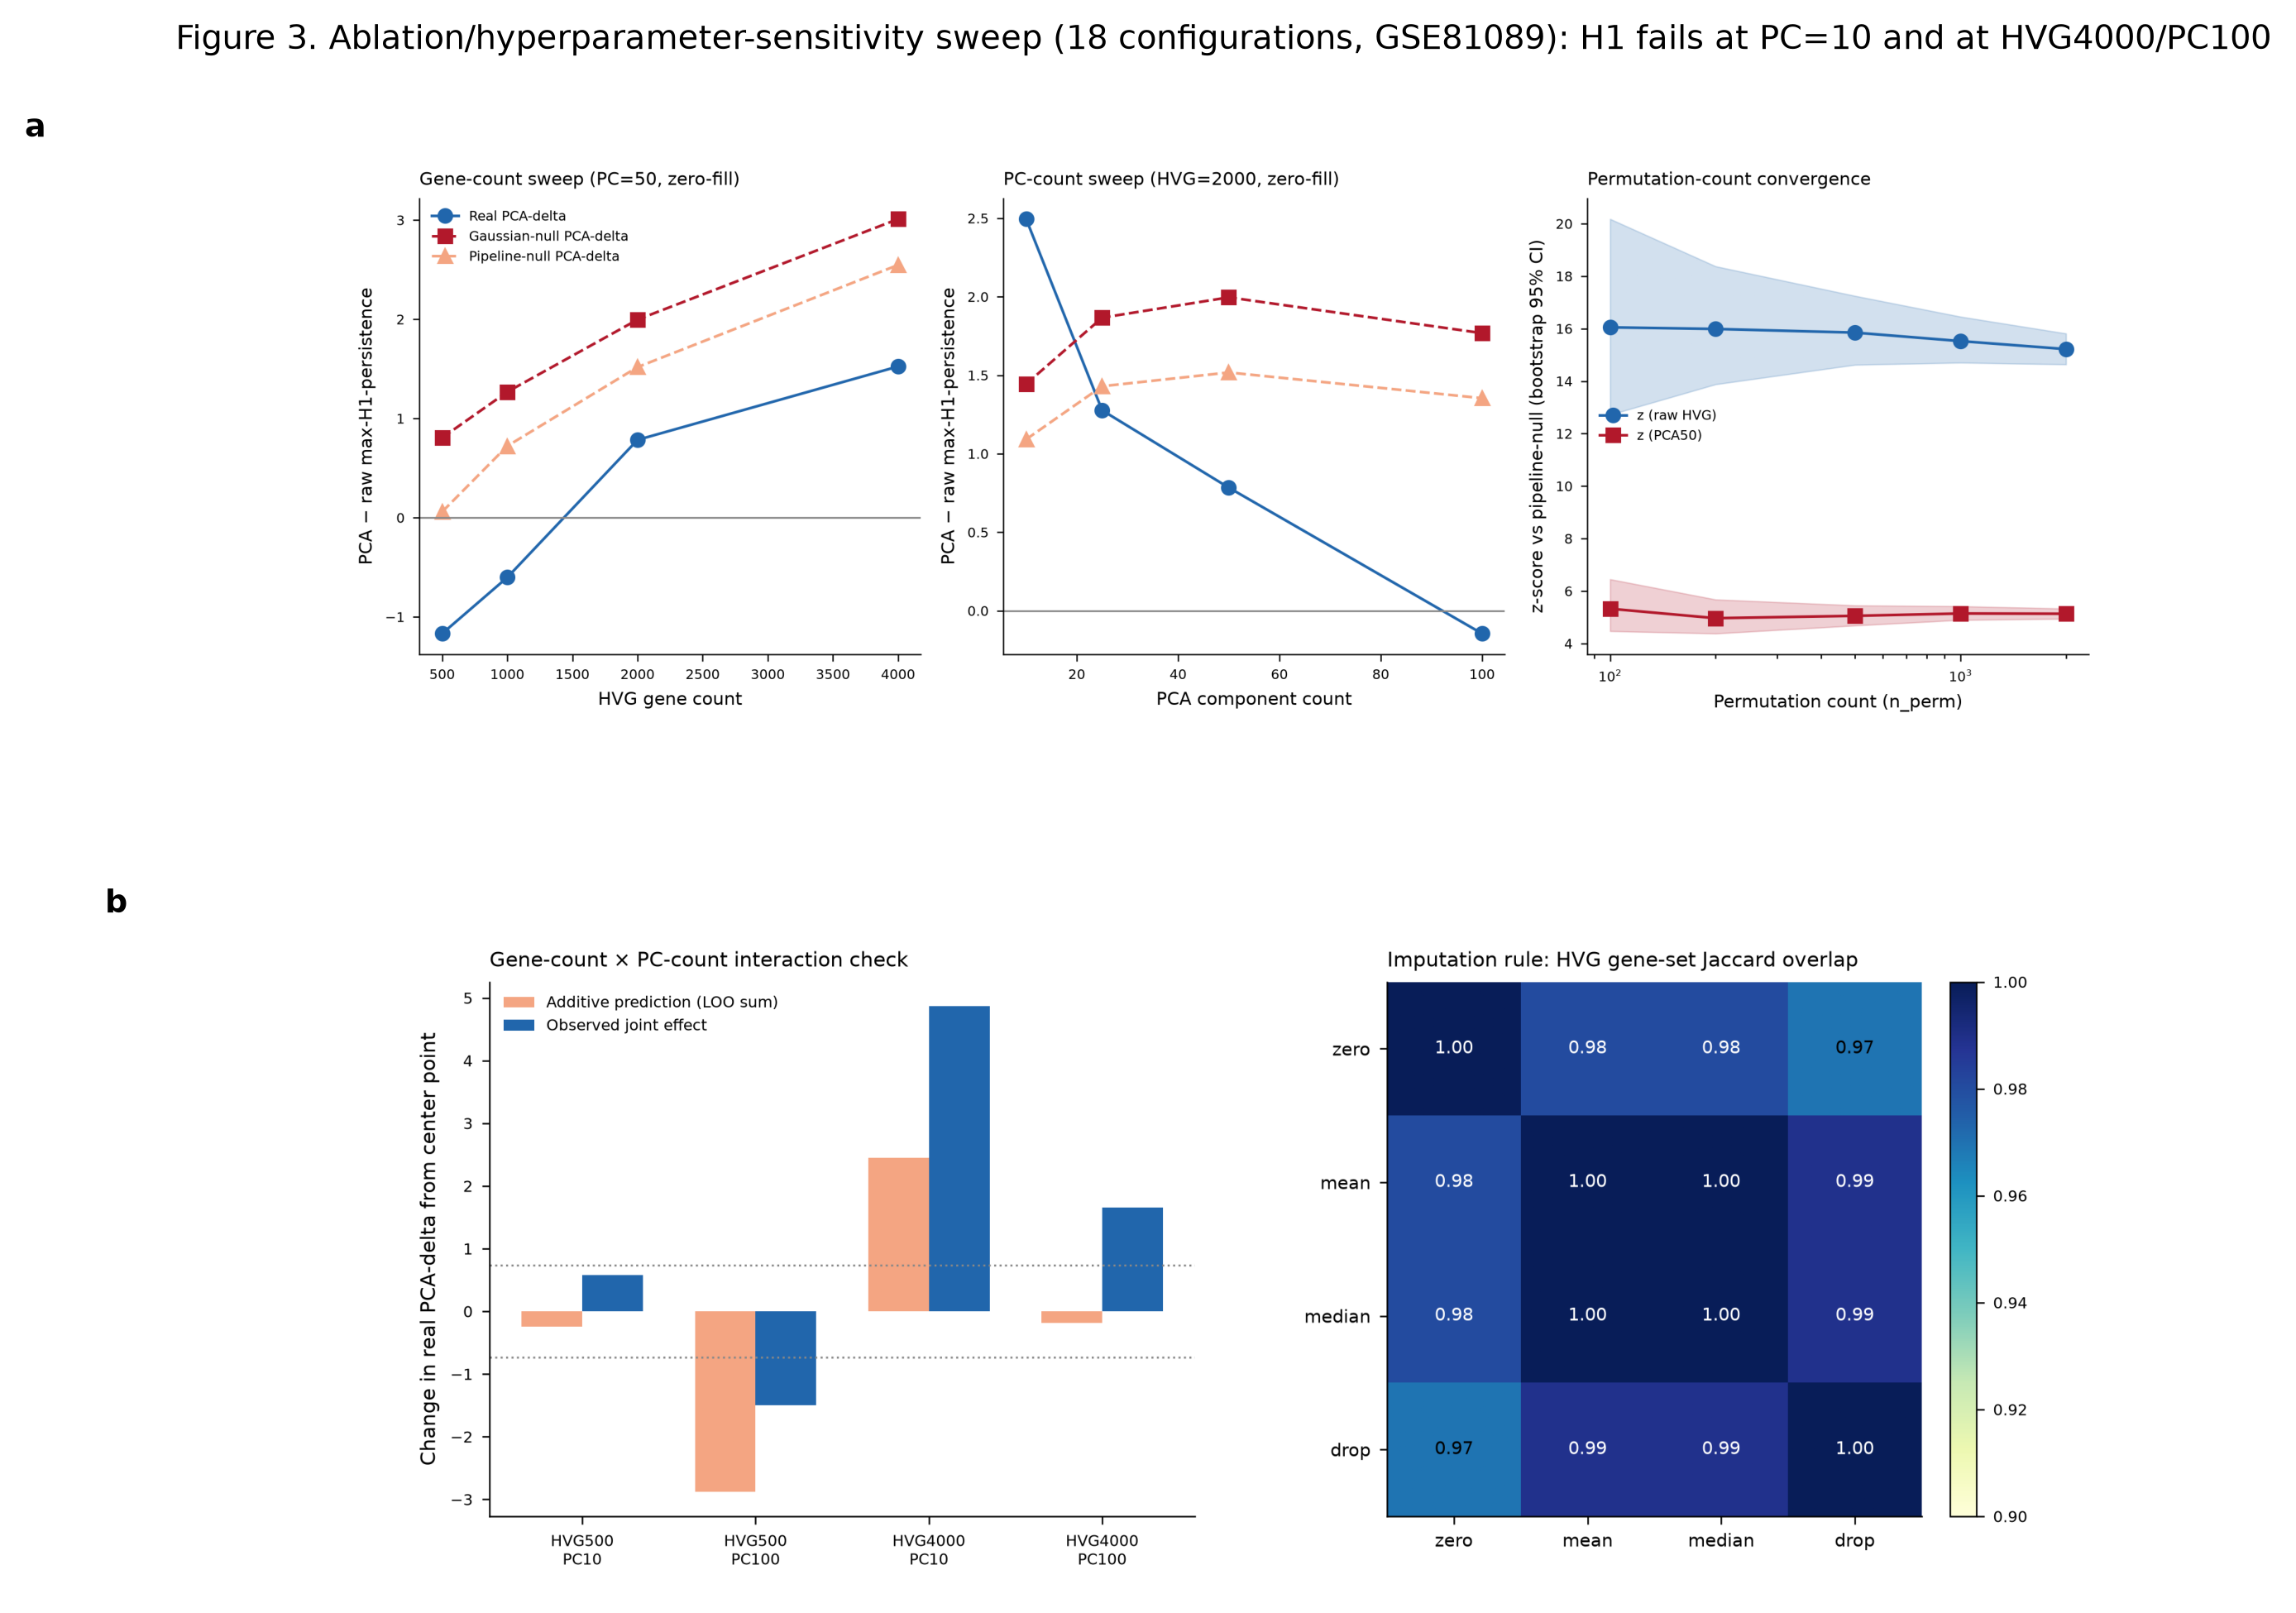
\includegraphics[width=0.95\textwidth]{figures/fig3_ablation_sensitivity.png}
\caption{\textbf{Ablation/hyperparameter-sensitivity sweep (18 configurations, pilot cohort GSE81089).} (a, left) Gene-count sweep at PC$=50$: real PCA-driven $\Delta$ (blue) crosses below zero at HVG$=500$ and again near HVG$=4000$ relative to the null $\Delta$s (red/orange), which remain positive throughout. (a, center) PC-count sweep at HVG$=2000$: real $\Delta$ exceeds both null $\Delta$s at PC$=10$, the dominant failure mode, then falls below both nulls from PC$=25$ onward. (a, right) Permutation-count convergence: $z$-scores vs.\ pipeline-symmetric null stabilize well before the pre-registered $n=2000$. (b, left) Gene-count $\times$ PC-count interaction check: observed joint effect (blue) vs.\ additive prediction (orange) at the four grid corners; all four corners show superadditive interaction. (b, right) Imputation-rule HVG gene-set Jaccard overlap: all pairwise overlaps $\geq0.97$.}
\label{fig:fig3}
\end{figure}

\subsection{Confound-attribution audit: pilot cohort (GSE81089)}
\label{sec:results-confound}

Having established that $H_1^{\text{stat}}$ (PCA-attribution) is robust at the pre-registered operating point in the pilot cohort, the confound-attribution audit (\Cref{sec:methods-confound}) asks a distinct question: is the residual topological signal that does survive both nulls at the pre-registered operating point attributable to the tumor/normal class-mean shift, or independent of it? \textbf{This audit has been completed, at the time of writing, only for the pilot cohort, GSE81089.} We report its result here scoped explicitly to this one cohort; whether it generalizes to the three replication cohorts is an open question (\Cref{fig:fig4}c).

In GSE81089, the tumor/normal class-mean-shift direction correlates strongly with PC1 ($r=0.865$) and a linear classifier recovers tumor/normal status from the top discriminant direction alone at $\mathrm{AUC}=0.9995$. Despite this, four independent lines of evidence indicate the $H_1$ topological signal is not a re-description of that class-mean shift, within this cohort:

\begin{enumerate}
\item \textbf{Within-class decomposition.} Restricting to the tumor-only subpopulation ($n=199/218$) reproduces the identical $\maxHone$ statistic (3.887) found in the full mixed population, with strong significance against both nulls ($z=23.0$ Gaussian, $z=14.5$ permutation). The normal-only subpopulation ($n=19$) shows no comparable signal ($\maxHone=0.405$).
\item \textbf{Within-stratum control.} Stratifying the tumor-only subpopulation into quartiles along the class-mean-shift direction, the signal survives in every quartile ($z=8.8$--$28.4$ against the matched Gaussian null), ruling out a signal concentrated only in samples closest to the normal population along that axis.
\item \textbf{Residualization control.} After projecting out the class-mean-shift direction, $\maxHone$ remains high (3.731, vs.\ 3.887 unresidualized) and significant against the Gaussian null ($z=31.1$); against the more conservative pipeline-permutation null the residualized signal is $z=2.97$ --- just under the pre-registered $z>3.0$ threshold, a partial rather than unambiguous pass. Critically, a classifier trained on the residualized data to recover tumor/normal status collapses from $\mathrm{AUC}=1.000$ (unresidualized) to $\mathrm{AUC}=0.094$ (a permutation test on this collapse gives $p=0.005$), confirming the confound direction was successfully removed.
\item \textbf{Block-bootstrap confidence interval.} A block-bootstrap 95\% CI on the residual signal-beyond-null quantity is $[1.37, 3.77]$, excluding zero.
\end{enumerate}

\begin{figure}[htbp]
\centering
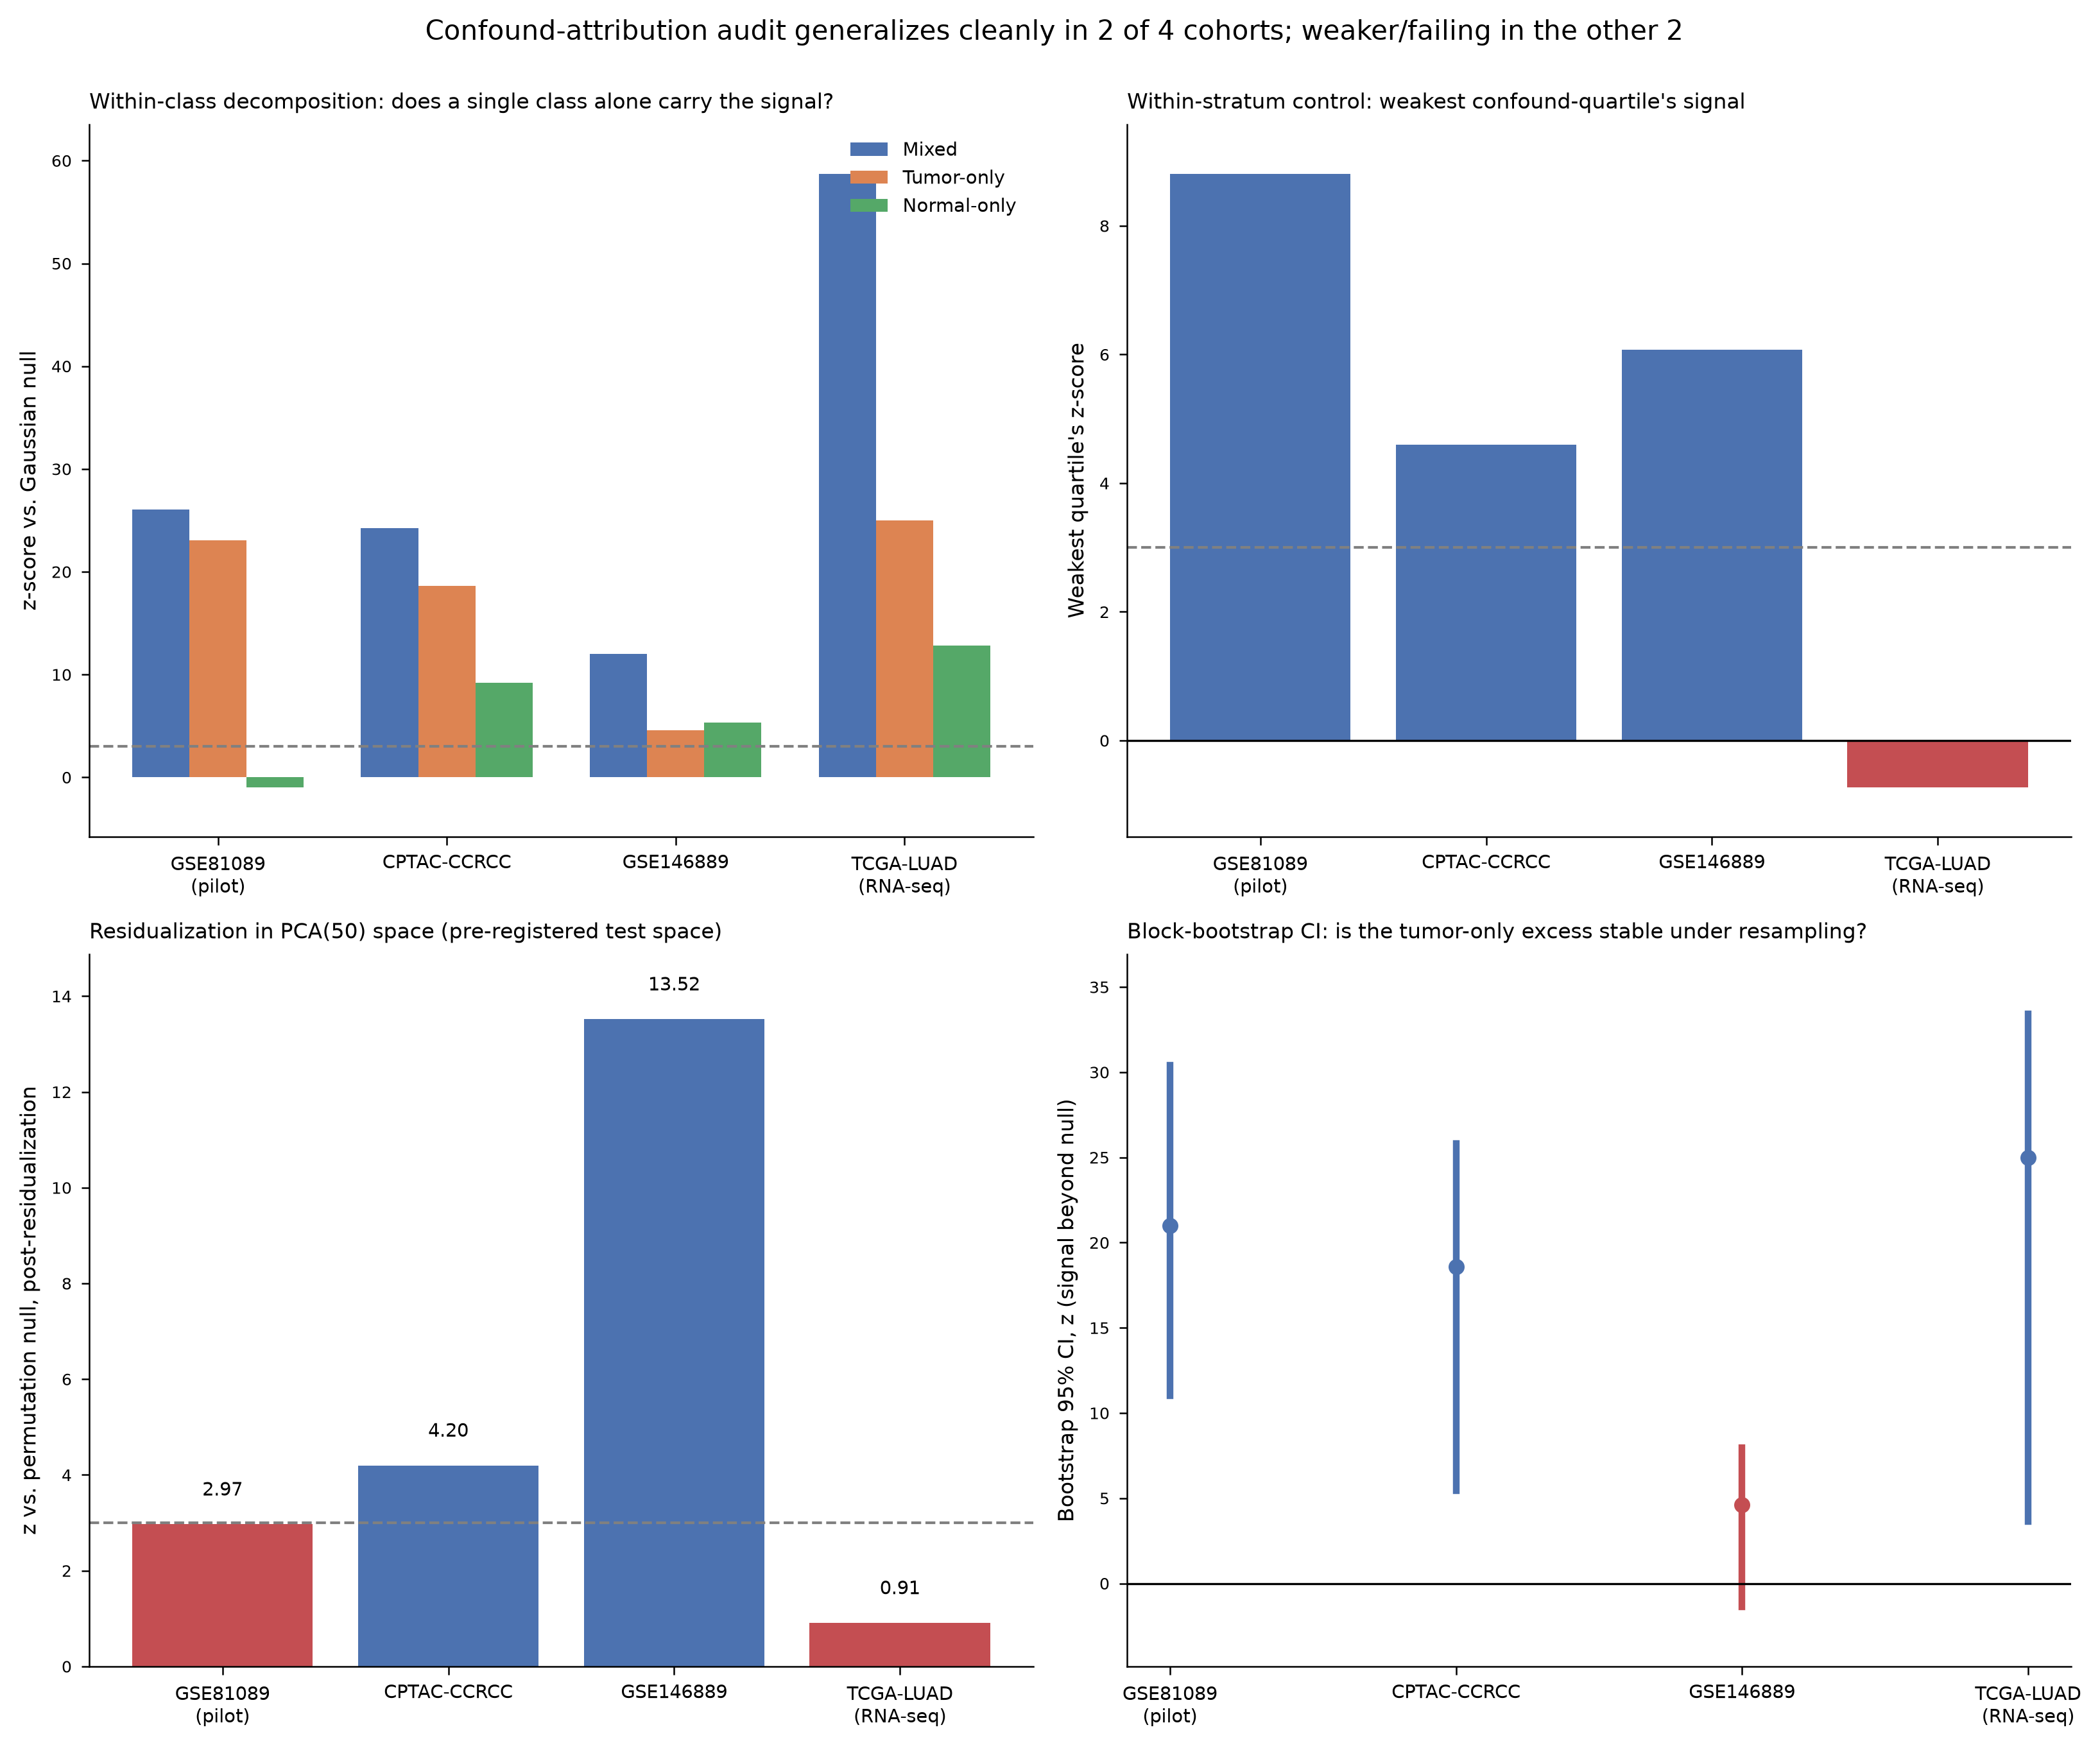
\includegraphics[width=0.92\textwidth]{figures/fig4_confound_audit.png}
\caption{\textbf{Confound-attribution audit across all four cohorts.} Dashed grey line marks the pre-registered $z=3.0$ threshold; bars/points below or crossing it are colored red. (a) Within-class decomposition: $z$-score (vs.\ Gaussian null) for the mixed population, tumor-only subset, and normal-only subset, in each cohort. GSE81089's underpowered normal-only arm ($n=19$) shows no excess; CPTAC-CCRCC's well-powered normal-only arm ($n=84$) does. (b) Within-stratum control: the \emph{weakest} confound-quartile's $z$-score in each cohort --- all clear threshold except TCGA-LUAD, where the least tumor-like quartile falls \emph{below} its own null mean. (c) Residualization in PCA(50) space --- the space this program's primary tests are run in --- against the more conservative permutation null: GSE81089 sits just at threshold ($z=2.97$), CPTAC-CCRCC and GSE146889 clear it, and TCGA-LUAD collapses to null-indistinguishable ($z=0.91$). (d) Block-bootstrap 95\% CI on the tumor-only signal-beyond-null ($z$-scale): GSE81089, CPTAC-CCRCC, and TCGA-LUAD exclude zero (TCGA-LUAD's lower bound is close to threshold); GSE146889 does not.}
\label{fig:fig4}
\end{figure}

\subsection{Confound-attribution audit: generalization to the three replication cohorts}
\label{sec:results-confound-generalization}

The same four-part audit protocol (\Cref{sec:methods-confound}) was subsequently applied, identically, to
GSE146889, CPTAC-CCRCC, and TCGA-LUAD (RNA-seq layer; the methylation layer was excluded because its
real PCA-space $\maxHone$ is already zero, so there is no signal to attribute). Each audit independently
re-verified its dataset's earlier pipeline numbers (real $\maxHone$, intrinsic dimension, classifier AUC)
to high precision before running any new test, confirming the reproduction was faithful. \Cref{tab:confound-crossdataset}
summarizes all four audits, including the pilot.

\begin{table}[htbp]
\centering
\small
\caption{Confound-attribution audit summary across all four cohorts. ``Within-class match'' asks whether a
single-class subset reproduces the mixed-population $\maxHone$ statistic; ``Within-stratum'' asks whether
every confound-quartile clears $z>3.0$; ``Residualization'' reports whether the aggregate signal survives
exact linear removal of the class-mean-shift direction (and, where relevant, in which feature space);
``Bootstrap CI'' reports whether the 95\% block-bootstrap CI on the signal-beyond-null excludes zero.}
\label{tab:confound-crossdataset}
\begin{tabular}{@{}p{2.6cm}p{2.6cm}p{2.3cm}p{3.6cm}p{2.6cm}p{2.6cm}@{}}
\toprule
Dataset & Within-class match & Within-stratum & Residualization & Bootstrap CI & Verdict \\
\midrule
GSE81089 (pilot) & Yes ($3.887=3.887$) & Yes ($z{=}8.8$--$28.4$) & Gaussian $z{=}31.1$; permutation $z{=}2.97$ (near-miss) & Yes, tumor-only $[1.37,3.77]$ & Genuine, tumor-scoped \\
CPTAC-CCRCC & Yes ($3.833=3.833$) & Yes ($z{=}4.6$--$11.3$) & Gaussian $z{=}36.5$; permutation $z{=}4.20$ (clears) & Yes, tumor-only $[0.83,3.96]$ & Genuine, extends to normal tissue \\
GSE146889 & \textbf{No} ($5.880$ vs.\ $7.564$, 78\%) & Yes ($z{=}6.1$--$23.6$)\footnotemark[1] & Clears aggregate stat ($z{=}14.4/13.5$) but dominant loop \emph{identity} changes & \textbf{No}, neither subset excludes 0 & Partially genuine, weaker \\
TCGA-LUAD (RNA-seq) & \textbf{No} ($4.596$ vs.\ $8.327$, 55\%) & \textbf{No} --- Q1 fails ($z{=}-0.73$) & Raw space survives but $=$ pre-existing normal-loop statistic; \textbf{PCA(50) space collapses} ($z{=}0.50/0.91$) & Marginal, lower bound $z{=}3.65$ & Mixed/weaker, fails in pre-registered space \\
\bottomrule
\end{tabular}
\vspace{2pt}
\footnotesize{\footnotemark[1]Quartiles here are not label-balanced (Q1 98\% normal, Q4 100\% tumor) because the classifier separates the classes cleanly along this exact projection.}
\end{table}

\textbf{Two of four cohorts (GSE81089, CPTAC-CCRCC) replicate the clean genuine-signal picture.}
CPTAC-CCRCC's audit reproduces every element of the pilot's decisive result: the tumor-only subset matches
the mixed-population statistic to six decimal places, every confound-quartile clears the significance bar,
and the residualized signal survives against \emph{both} nulls with more room than the pilot itself
($z=4.20$ vs.\ the pilot's near-miss $z=2.97$ against the permutation null). CPTAC-CCRCC additionally has a
well-powered normal-only arm ($n=84$, vs.\ the pilot's underpowered $n=19$) that also clears the null
threshold ($z=9.2$ Gaussian, $z=14.2$ permutation) --- a result the pilot could not establish either way,
extending rather than merely replicating the confound-independence finding to a second tissue compartment.

\textbf{The other two cohorts (GSE146889, TCGA-LUAD) do not.} GSE146889 passes the within-stratum control
and the residualization control at the level of the aggregate $\maxHone$ scalar, but fails the two controls
that gave the pilot its most decisive, assumption-light evidence: neither the tumor-only nor the
normal-only subset reproduces the mixed-population magnitude, and neither subset's bootstrap CI on the
signal-beyond-null excludes zero. Moreover, while the aggregate statistic survives residualization, the
\emph{specific dominant loop} does not --- a different set of 22 samples, at a near-baseline tumor/normal
composition (Fisher $p=0.65$), replaces the original 45-sample, tumor-enriched loop (Fisher $p=2.9\times10^{-9}$,
\Cref{sec:results-confound-crossdataset}) as the top persistence feature once the confound is removed. The
aggregate scalar surviving does not mean the same geometric object survives.

TCGA-LUAD shows the most direct counter-example to a general confound-independence claim. Its within-stratum
control fails outright in the least tumor-like quartile (observed $\maxHone$ falls \emph{below} its own null
mean, $z=-0.73$), and --- most consequentially --- residualization in \textbf{PCA(50) space, the exact space
this program's entire pre-registered test family and the pilot's own headline comparison are conducted in},
collapses the signal to null-indistinguishable ($z=0.50$ Gaussian, $z=0.91$ permutation). A signal does
survive residualization in raw $2000$-gene space, but a structural check shows this raw-space value is
\emph{numerically identical} to the pre-residualization normal-only statistic (an exact-invariance property
of how a constant per-class linear shift interacts with within-class pairwise distances) --- it reflects
pre-existing intra-normal-tissue structure passing through unchanged, not a demonstrated tumor-associated
signal surviving the control. This raw-space survival therefore does not rescue the PCA-space finding.

\Cref{fig:fig4} panel (c), previously a placeholder, now shows all four cohorts' verdicts side by side.

\subsection{Honest cross-dataset confound-attribution pattern}

Across all four cohorts, the underlying $H_0^{\text{stat}}$ real-vs-null test (\Cref{tab:h0-crossdataset})
remains robust in every case --- the confound audit's mixed and partial findings concern \emph{whether an
already-established signal is a confound artifact}, not whether the signal exists relative to null at all.
What varies across cohorts is how much of that signal survives confound control, and specifically whether
it survives in the pre-registered PCA(50) space where the program's primary claims are made. The pattern is
2-of-4 clean, 2-of-4 partial-to-failing, with no single covariate (modality, tissue homogeneity, or
confound-variance share) cleanly separating the two groups: GSE81089 and TCGA-LUAD are both RNA-seq, yet
land on opposite sides; CPTAC-CCRCC (proteomics) and GSE146889 (RNA-seq, mixed tissue) are not obviously
more similar to their respective clean/partial partners than to each other. We report this as a genuine,
unresolved heterogeneity rather than force a single verdict onto the full replication family.

\section{Discussion}
\label{sec:discussion}

\TODO{This section is deliberately left as a placeholder. The final discussion and scope statement depend on the outcome of the confound-attribution audit's generalization to GSE146889, CPTAC-CCRCC, and TCGA-LUAD (\Cref{sec:methods-confound}, \Cref{sec:results-confound}), which is in progress and has not yet reported back at the time of writing. Do not draft a synthesis here that assumes a particular outcome for those three audits --- the pilot cohort's finding (confound-independence of the $H_1$ signal, scoped strictly to GSE81089) must not be extrapolated to a general or cross-cohort claim until it is either replicated or refuted in each of the other three cohorts. Note in particular that GSE146889's own cross-check (\Cref{sec:results-confound-crossdataset}) already shows a structural difference from the pilot --- a significantly tumor-enriched dominant $H_1$ loop --- that is a specific, concrete reason the pilot's confound-independence result might not transfer there; the synthesis phase should treat this as a live possibility to be resolved by the pending audit, not dismissed in advance.}

\TODO{Once the three remaining confound audits complete, this section should address at minimum: (i) what the complete cross-cohort pattern implies about whether the pilot's confound-independence finding is a general property of the pipeline or a property specific to the pilot cohort's biology/data-collection process; (ii) how the ablation sweep's identified failure boundaries (PC=10; HVG=4000/PC=100) interact with the confound-audit's scope --- e.g., whether a dataset that fails the ablation boundary conditions should be interpreted differently in the confound audit; (iii) an honest statement of what this program does and does not establish about the general relationship between PCA and persistent-homology-based topological claims in omics data, calibrated against the actual evidence gathered rather than the most publishable-sounding interpretation of it; (iv) limitations, including the reliance on a single primary test statistic (max-$H_1$ persistence) rather than a full persistence-diagram distance, the restriction to five cohorts across a still-limited set of tissue types, and the fact that the ablation sweep was run only on the pilot cohort and has not itself been cross-validated on the replication cohorts.}


\printbibliography

\end{document}
